\documentclass[conference]{IEEEtran}
\IEEEoverridecommandlockouts
% The preceding line is only needed to identify funding in the first footnote. If that is unneeded, please comment it out.
\usepackage{cite}
\usepackage{amsmath,amssymb,amsfonts}
\usepackage{algorithmic}
\usepackage{graphicx}
\usepackage{textcomp}
\usepackage{xcolor}
\usepackage{multirow}
\usepackage{array}
\usepackage{listings}
\newcolumntype{L}[1]{>{\raggedright\let\newline\\\arraybackslash\hspace{0pt}}m{#1}}

\def\BibTeX{{\rm B\kern-.05em{\sc i\kern-.025em b}\kern-.08em
    T\kern-.1667em\lower.7ex\hbox{E}\kern-.125emX}}
\usepackage{subcaption}    

\begin{document}
\bibliographystyle{IEEEtran}


\title{Using the Graphcore IPU for traditional HPC applications\\
\thanks{This work was partly funded by the Engineering and Physical Sciences Research Council (EPSRC) via the Advanced Simulation and Modelling of Virtual Systems (ASiMoV) project, EP/S005072/1}
}

\author{\IEEEauthorblockN{Thorben Louw, Simon McIntosh-Smith}
\IEEEauthorblockA{\textit{Dept. of Computer Science} \\
\textit{University of Bristol}\\
Bristol, United Kingdom \\
\{thorben.louw.2019, S.McIntosh-Smith\}@bristol.ac.uk
}}


\maketitle

\begin{abstract}
 The increase in machine learning workloads means that AI accelerators are expected to become common in supercomputers, evoking considerable interest in the scientific high-performance computing (HPC) community about how these devices might also be exploited for traditional HPC workloads. In this paper, we report our early results using the Graphcore Intelligence Processing Unit (IPU) for stencil computations on structured grid problems, which are used for solvers for differential equations in domains such as computational fluid dynamics.
 We characterise the IPU's performance by presenting both STREAM memory bandwidth benchmark results and a Roofline performance model.
 %, and show that the Roofline model is unable to convey a fundamental performance ceiling on this platform arising from its Bulk Synchronous Parallel and distributed memory design.
 Using two example applications (the Gaussian Blur filter and a 2D Lattice Boltzmann fluid simulation), we discuss the challenges encountered during this first known IPU implementation of structured grid stencils.
 We demonstrate that the IPU and its low-level programming framework, Poplar, expose sufficient programmability to express these HPC problems, and achieve performance comparable to that of modern GPUs.

\end{abstract}

\begin{IEEEkeywords}
accelerator, HPC, structured grid, stencil, heterogeneous computing
\end{IEEEkeywords}

\section{Introduction}
Recent progress in machine learning (ML) has created an exponential growth in demand for computational resources 
\cite{openai-power-analysis}, with a corresponding increase in energy use for computation. This demand, coming at a time when Moore's Law has slowed and Dennard Scaling no longer holds, has led to the development of  energy-efficient hardware accelerator devices for artificial intelligence (AI) processing. 

Devices targeting the edge computing or inference-only markets may have limited support for floating point computation. But devices designed for accelerating ML training often support 32-bit floating point computation. They have large amounts of on-chip memory for holding weights without resorting to transfers from host DRAM and include custom hardware for common ML operations (e.g. matrix engines). These capabilities have let to interest in exploiting AI devices for traditional scientific HPC \cite{domke2020matrix, cerebras}, and research into mixed-precision implementations of numerical solver algorithms \cite{mixed-precision-sim}. 

An example of an AI accelerator that supports floating point computation is Graphcore’s Intelligence Processsing Unit (IPU). The IPU has large amounts of fast on-chip SRAM (static random-access memory), distributed as 256KiB local memories for each of its 1216 cores. There is no global memory, and cores must share data by passing messages over the IPU's high-bandwidth, all-to-all interconnect. IPUs incorporate specialised hardware for common machine learning operations such as convolutions and matrix multiplication. Most alluringly for HPC developers, the IPU can be programmed at a low-level by using its C++ framework, Poplar, making it possible to implement HPC applications without having to shoehorn them into higher-level ML frameworks. 

The IPU's design is based on the Bulk Synchronous Parallel (BSP) model of computation \cite{Valiant1990} that Poplar combines with a tensor-based computational dataflow graph paradigm familiar from ML frameworks such as Tensorflow. The Poplar graph compiler lowers the graph representation of a program into optimised communication and computation primitives, while allowing custom code to access all of the IPU's functionality.

In this work, we implement two structured grid stencil applications (a Gaussian Blur image filter and a 2D Lattice Boltzmann fluid simulation) to demonstrate the feasibility of implementing HPC applications on the IPU. We achieve very good performance, far exceeding that of our comparison implementation on 48 CPU cores, and comparable with the results we see on the NVIDIA V100 GPU. We present our performance modelling in the form of STREAM memory bandwidth benchmarks and a Roofline model for the IPU.

In contrast to the large body of research concerned with accelerating HPC applications on GPUs, very little has been published for the IPU. We use results from Jia, Tillman, Maggioni and Scarpazza's detailed micro-benchmarking study of the IPU’s performance~\cite{CitadelPaper} in this paper.  Other known work concerns bundle adjustment in computer vision ~\cite{Ortiz2020}, performance for deep learning-based image applications~\cite{kacher2020graphcore} and applying the IPU for machine learning in particle physics~\cite{particle-physics-ipu}. To the best of our knowledge, this work represents the first application of this architecture for structured grid problems and ``traditional'' HPC.
 
% The rest of this paper is structured as follows: In Section\-\ref{sec:ipu-overview}, we give a brief overview of the IPU and its programming framework, Poplar. In Section\-\ref{sec:structured-grid}, we discuss the implementation of structured grid applications on the IPU. We then present a memory bandwidth characterisation (STREAM) and a Roofline model for the IPU in Section\-\ref{sec:performance}, and discuss the implementation of two example application in Section\-\ref{sec:examples} before discussing our experience, concludinrk and g.

\section{The Graphcore IPU and Poplar programming framework}
\label{sec:ipu-overview}
The Graphcore MK-1 IPU processor consists of 1216 cores, each with its own 256KiB local high-bandwidth, low-latency SRAM memory. Together, a core and its memory are termed a ``tile''. There are no other caches, and there is no global shared memory between cores.  Tiles can exchange data using a very fast all-to-all, on-chip interconnect (theoretically 8 TB/s). For ML applications, many models' weights can be held entirely in on-chip memory.  

The IPU supports both 32-bit (single) and 16-bit (IEEE754 half) precision floating point numbers, but  not 64-bit (double) precision. Cores have specialised ML operation hardware, such as Accumulating Matrix Product (AMP) units and hardware for efficient convolutions. Being able to use these operations from HPC programs makes the IPU very attractive, since they are also common in scientific code. 

Every core supports six hardware worker threads, which run in a time-sliced fashion to hide instruction latency. Most instructions complete in one ``thread cycle''. 

MK-1 IPUs are available on dual-IPU C2 cards connected to a host over PCIe4 x16. Systems scale to multiple IPUs using a fast custom inter-IPU link that allows communication without involving the host. 

Each IPU uses approximately 150W of power -- significantly less than contemporary HPC GPUs (cf. 250W TDP for the NVIDIA V100 \cite{CitadelPaper}).

Graphcore recently announced a more powerful MK2 IPU, with 3x the SRAM and more cores, but we did not have access to it for this work.

\subsection{Programming framework}
\label{sec:poplar}
IPUs are easily integrated with common ML frameworks such as Tensorflow and PyTorch, but Graphcore also provides low-level programmability via its Poplar C++ framework. In contrast to the scant public details available about the software stacks of other emerging accelerators, Graphcore's libraries are open source and SDK documentation is publicly available~\cite{graphcore-docs}.

Poplar programs build a computational dataflow graph in which nodes represent computation and edges represent the flow of data, modelled as tensors (typed multidimensional arrays). Poplar graphs support full control flow such as iteration and branching, but are restricted to be static, and tensor dimensions must be known at (graph) compile time. Tensors are a conceptual construct that must be mapped to actual tile memories during graph construction, with a tensor potentially partitioned over many tiles.

Poplar programs follow Valiant's Bulk-Synchronous Parallel (BSP) model of computation~\cite{Valiant1990}, in which serial supersteps are made up of parallel execution, exchange and synchronisation phases. This allows concurrency hazards to be avoided, and the compiler is able to implicitly schedule and optimise the communication (``exchanges'') of tensor regions both between IPUs and between each IPU's tiles. In Poplar, the BSP style is enforced by grouping operations into ``compute sets'', with restrictions on reading and writing the same tensor regions from different workers in the same compute phase.

While a large number of optimised operations on tensors (e.g. matrix multiplication, reductions, padding) are available through Poplar's libraries, custom operations called ``vertexes'' can be written in standard C++. Vertexes form the primary mechanism we will exploit for HPC purposes. Example code for a Vertex is shown in Appendix~B.

Vertexes are unaware of either the tensor abstraction or the graph -- they are small C++ objects defining methods which operate on primitive C++ types. Class members defined as special \texttt{Input}, \texttt{Output} or \texttt{InOut} types define a vertex's interface for wiring into the dataflow graph. Vertexes must be explicitly mapped to compute sets and tiles during program construction. 

Wiring up vertexes to tensors in the graph tells the graph compiler when data needs to be sent between tiles, and it automatically generates the required messages. In addition, when a vertex specifies memory alignments, or input and output tensors are manipulated during wiring (e.g. reshaping, slicing), data rearrangements are generated by the graph compiler, and these are not under the programmer's explicit control. 

Scaling to multiple IPUs is made relatively transparent by Poplar: by selecting a ``multi-IPU'' device, the programmer is presented with a virtual device with the requested multiple of tiles, and the compiler generates any necessary inter-IPU communication.

\section{Structured Grids and Stencils}
\label{sec:structured-grids}
Structured grids are one of the classes described by Asanovi\'c \emph{et~al} in their characterisation of the computational requirements of different parallel programming problems~\cite{dwarves}. They are commonly used in solvers for differential equations, such as those underpinning heat and fluid simulations.

In these applications, the domain under investigation is discretised onto a regular grid of cells. The structured layout means that a cell's neighbours can be located in a simple data structure using offset calculations, resulting in regular, predictable memory access patterns. This is in contrast to using \textit{un}structured grids, where neighbours are described using (sparse) graphs. 

% Discretisation of the differential equation on the grid results in formulas which update the value of a variable of interest based on a weighted combination of values of neighbouring cells. When these are represented as edge weights in a graph, and weighted adjancency matrix is constructed, a large often diagonally-dominant coefficient matrix A in a linear system Ax=b.

\subsection{Stencils}
Systems of linear equations which arise from the finite difference approximation of differential equations onto a structured grid are characterised by a large, sparse coefficient matrix with low bandwidth. In some cases, it is possible to avoid representing the coefficients altogether and rely on matrix-free methods for the sparse matrix-dense vector part of the solution.

Matrix-free computation uses a \textit{stencil}, which defines the regular pattern of computation that is applied to the local neighbourhood of each cell to determine the next value at each time step. 

% If the domain is decomposed into rectangles or volumes and shared among workers, each worker’s region of computation is largely exclusive. Only cells on the boundaries between workers (the “halo regions”) need to be shared between workers. This allows for efficient re-use of shared memory on GPU devices and good use of local caches between cores of the same CPU. 

% In parallel implementations with distributed memories, the halo regions need to be communicated between neighbours, typically using MPI.

% A large body of existing work describes optimisations of stencil implementations. Given the memory bandwidth-bound nature of stencils, most of these optimisations focus on improving cache locality within a node, and include spatial and temporal blocking and polyhedral loop tiling to maximise data reuse in caches and registers. Appropriate data layout (padding, alignment, structure of array vs array of structure, row or column orientation). and exploiting vectorisation. 

% Distributed parallel implementations exploit optimisations such as overlapping computation and communication by performing inner region computations while halos are being exchanged, exchanging wide halos that hide communication latency by redundantly recomputing boundary regions and communicating less frequently, and performing halo exchange in optimised “two-wave” techniques to minimise the number of messages sent. 

\subsection{Implementation on the IPU}
 Implementing structured grids on the IPU means addressing a number of concerns:

\paragraph{Representing grids and cells}
Tensors form a natural representation of regular 2D and 3D grids of rectangular cells, and allow multi-valued cells to be represented with an extra tensor dimension.

\paragraph{Partitioning and load balancing}
The grid tensor is too large for any one tile's memory, so it must be partitioned by placing slices of the tensor on different tiles. 

Partitioning overlaps with a load balancing concern: because we want to minimise exchanges, a core should operate on the cells in its local memory where possible, meaning that the size a tile's tensor partition defines the amount of work the tile will do. Achieving a good load balance on the IPU is crucial, because the BSP design means that execution is limited by the most heavily loaded tile. 

Partitions should be small enough to allow using as many tiles as possible, yet not so small that the benefits of parallelism are outweighed by any increased communication between tiles. We also want to sub-partition work equally between the core's 6 worker threads, and constrain sub-partitions to fall along tensor slice dimensions for simplicity of implementation.

% In light of the above constraints, we only considered spatial decomposition strategies, not spatio-temporal decompositions such as diamond tiling~\cite{bandishti2012tiling}. Spatio-temporal schemes are largely aimed at achieving better cache locality, which is not a concern for the cacheless IPU.

Our simple strategy lays out the IPU tiles in a grid whose dimensions best match the aspect ratio of the domain (e.g. a 2048x2048 grid is mapped onto the 1216 tiles laid out in a 38x32 configuration) and divides work as equally as possible in each dimension. This works well for structured grid applications where each cell's work has equal cost. More complex applications will need to use more advanced graph partitioning algorithms.

When the grid is so large that it does not fit in the combined IPUs' memories, the domain must be decomposed into overlapping sub-grids in the host memory, each of which is processed in turn on the IPUs, meaning that the bottleneck becomes the PCIe connection to the host (64 GB/s). We do not consider optimisations for these large problems in this work.

\paragraph{Halo exchange}
Decomposed stencil problems need to access the ``halo'' of boundary cells stored on surrounding neighbour tiles, as shown in Fig.~\-\ref{fig:halo-exchange}. These cells must be exchanged between BSP compute phases (``halo exchange'').

\begin{figure}[htbp]
\centerline{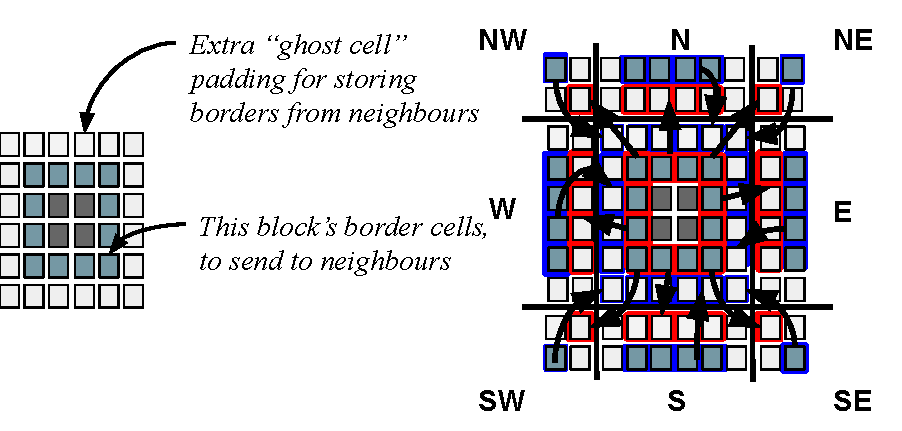
\includegraphics[width=0.5\textwidth]{halo-exchange.pdf}}
\caption{Halo exchange between a cell and its 8 neighbours.}
\label{fig:halo-exchange}
\end{figure}

We experimented with a variety of halo exchange patterns and implementations on the IPU, but our best performance was achieved by implicitly letting the compiler generate the necessary exchanges. To prompt this communication, a vertex's halo regions are wired up to tensor slices on remote tiles.

A succinct vertex implementation assumes its input data is packed in one contiguous area of memory (so that loops only need to consider one underlying data structure), which we achieve by slicing, concatenating and flattening tensors when vertexes are wired up. Unfortunately this elegant solution causes the graph compiler to introduce \textit{data rearrangements}. Even when no halo exchange takes place, data rearrangements will also occur if the vertex specifies constraints on inputs or outputs (e.g. alignment, or specifies a memory bank). 

Other viable options for halo-exchange implementations either pass separate, non-concatenated input tensors to the vertex, resulting in a large number of special loop cases; or use explicit copy steps in the graph to duplicate halo regions.

%\footnote{Explicit halo exchange approaches depend on a compiler bug fix which will only become available an SDK version after 1.3.0}

% As an alternative, the vertex interface can have separate inputs for the various tensor regions that make up the halo (i.e. 9 inputs instead of 1). This results in complex vertex implementations and complex wiring code. Performance better, but best left to an auto-generated approach.

We do not communicate halos which are more than one cell wide. Sending wider halos is a common optimisation in systems where communication is costly and can be overlapped with communication (see e.g. ~\cite{palmer2002efficient}), but the high bandwidth of the IPU's exchange and the synchronisations in the BSP model reduce the advantages of doing so for the IPU.

\paragraph{Data access patterns}
The next timestep value of a cell depends on the previous timestep values of its neighbourhood. This means we cannot do in-place updates of cell values, but must hold temporary copies of at least some parts of the grid partition during computation. Poplar adds a further data access constraint that tensor regions cannot be read and written by two different vertexes in the same compute set. 

To overcome these constraints, we use a double-buffered scheme with two tensors for storing the grid. We read from tensor A and write to tensor B in one compute set, and read from tensor B and write to tensor A in the next compute set. This approach doubles the amount of required memory.

Since the IPU has no cache, performance is less dependent on the order in which memory locations are accessed than on a CPU: column- vs row-major layout, stride, and issues of coalesced access between threads are not important. The only optimisation which encourages a certain layout is that we can use the IPU's 64-bit SIMD instructions to perform calculations on pairs of 32-bit (``\texttt{float2}'') numbers, or quads of 16-bit (``\texttt{half4}'') numbers in a single cycle.  Case-by-base considerations for exploiting these vector instructions will determine whether an application uses array-of-structures (AoS) or structure-of-array (SoA) layouts to store cell contents. For example, in the Gaussian Blur example in Section \ref{sec:gaussian-blur}, we use AoS layout and four-wide SIMD instructions to process all four channels of pixel intensities simultaneously.

Using vectorised data types requires that data is aligned at natural boundaries, which may incur a data rearrangement cost that outweighs the benefit of vectorisation, so must be measured on a case-by-case basis.

\paragraph{Optimisations}
Stencil computations perform very few floating point operations (FLOPs) relative to the amount of memory accessed, making them memory bandwidth bound on most architectures. Hence, while a large body of work exists describing stencil optimisations (e.g. ~\cite{datta-et-al, maranushi-and-makino, tiling-stencils-for-max-parallel,kamil2006implicit}), much of this work focuses on improving cache locality to increase the operational intensity of kernels. As a result, few of these common optimisations apply for the cacheless IPU with its high local memory bandwidth.

Without resorting to assembly code, we found that the only ``easy win'' optimisations involved aligning memory, using vectorised SIMD instructions, unrolling loops, and exploiting special hardware through vendor-provided primitive operations on tensors. The more optimisations we apply manually, the less portable the code becomes. For kernels optimised in assembly, one can interleave memory and floating point instructions, use special instructions that perform simultaneous load-stores, and make use of counter-free loop instructions. Currently the \texttt{popc} compiler does not generate these automatically. 

% Extensions to the Roofline model have been proposed for cache-based architectures \cite{Ilic}, memory latency \cite{}, out-of-order execution \cite{}, energy use and communication costs \cite{}.  

% We found the Roofline model to be less useful for the IPU than for architectures with a hierarchy of caches. 

% Firstly, for the cacheless IPU, every memory access counts towards the OI and it is not possible to use caches to decrease the memory accesses. 
% Secondly, vector widths are low. (64-bit)
% Thirdly, memory isn't that simple. Costs of data rearrangements dominate. 
% [TODO: Don't duplicate what you say about performance]


% The cacheless IPU offers few options for increasing the operational intensity of a kernel other than through choosing vector instructions (e.g. processing a \texttt{half4} in one instruction rather than 4 \texttt{half}s in 4 instructions.) or decreasing memory instructions by using simultaneous load-stores, but as we have seen, this requires hand-optimisation of code or writing assembly.

% Can use float16 instead of float. 

% Stencil kernels typically have very low operational intensity, making them memory-bandwidth bound on most architectures. 


% We use this to construct Roofline models of the IPU’s performance. Problems: there’s no cache. We haven’t modelled the impact of “data rearrangements” [YOU NEED TO HAVE INTRODUCED DATA REARRANGEMENTS]

% Roofline models for architectures with caches count the number of loads and stores from ‘main memory’ to calculate operational intensity. Since every load and store is ‘from main memory’ on the IPU, and there are relatively few registers (with no large performance advantage for registers vs memory), the number of loads and stores is high. Very low operational intensity. From the model, at low intensity, the performance (FLOPs) will be limited by memory bandwidth. Few ways to address operational intensity on the IPU.

\section{Memory-bandwidth characterisation of the IPU}
\label{sec:performance}
Graphcore's marketing material lists the IPU's theoretical memory bandwidth as 45 TB/s. However, Jia, Tillman, Maggioni and Scarpazza ~\cite[p. 26]{CitadelPaper} calculate the IPU’s theoretical maximum aggregate read memory bandwidth as 31.1 TB/s (assuming all cores issue a 16-byte read instruction on every clock cycle, while running at maximum clock frequency), but note that less-than-perfect load instruction density will achieve only a fraction of this. These impressive numbers are an order of magnitude greater than the HBM2 memory on the contemporary NVIDIA A100, and are achieved in the IPU's design by placing on-chip SRAM physically close to each core. Unfortunately, theoretical memory bandwidth is rarely a useful guide to the achievable sustainable memory bandwidth that developers should expect. 

\subsection{STREAM}
Measuring actual achievable bandwidth is the aim of the BabelSTREAM benchmark suite~\cite{babelstream}, originally designed for GPUs, and since applied to CPU caches in~\cite{babelstream-cache}. Notably, one of the kernels in BabelSTREAM is the well-known STREAM benchmark by McCalpin~\cite{stream}, which is used as the memory bandwidth ceiling when constructing Roofline performance models. 

In this work, we implemented BabelSTREAM for the IPU using two approaches: naive C++ kernels with no explicit optimisations; and a combination of optimised C++ and Poplar primitives such as scaled, in-place addition. We also compared these results with an assembly implementation of STREAM provided by Graphcore. The results are shown in Table\ \ref{tab:STREAM}.


\begin{table}[htbp]
\caption{STREAM Triad kernel results for 3 implementations of BabelSTREAM on the IPU}
\begin{center}
\begin{tabular}{|c|l|r|}
\hline
\textbf{Precision}&\textbf{Implementation}&\textbf{Bandwidth} \\ 
\cline{3-3}
&& \textbf{\textit{GB/s}}\\
\hline
\multirow{3}{*}{32-bit} & C++ (naive) & 3,726 \\
& optimised/vendor primitives&7,261\\
&Assembly$^{\mathrm{a}}$&12,420\\
\hline
\multirow{2}{*}{16-bit}& C++ (naive) &1,488  \\
& optimised/vendor primitives & 7,490  \\
\hline
\multicolumn{3}{l}{$^{\mathrm{a}}$Provided by Graphcore.}
\end{tabular}
\label{tab:STREAM}
\end{center}
\end{table}



% \begin{table}[htbp]
% \caption{Comparison of IPU, GPU and CPU memory hierarchies.}
% \begin{center}
% \begin{tabular}{|c|l|r|r|r|r|}
% \hline
% \textbf{Platform}&\textbf{Memory}&\textbf{Size}&\textbf{Latency}&\textbf{Bandwidth} \\ \cline{4-5}
% & & & \textbf{\textit{ns}} & \textbf{\textit{GB/s)}} \\
% \hline
% IPU & SRAM & 304 MiB & 3.75 & 7,490--12,420 \\
% \hline
% \textit{GPU:}& L1/shared & 10 MiB & 11.9--20.1&  12,080  \\
% NVIDIA V100& L2 & 6 MiB & 121  &2,996 \\
% & HBM-2 & 16 GiB &  $\sim$1000&   828\\
% \hline
% \textit{CPU:}& L1 & 1.5MiB  & 1.48 & 12,875\\
% Intel Skylake& L2 & 48 MiB  & 4.44 & 4,474\\
% (2x 24 cores) & L3 & 66 MiB & 18.5--25.9 & ???\\
%  & DRAM & 768 GiB & $\sim$70 &  215\\
% \hline
% \end{tabular}
% \label{tab:cache-bandwidth}
% \end{center}
% \end{table}

The naive kernels achieved a disappointing fraction (approx. 12\%) of the theoretical memory bandwidth, confirming the findings in~\cite{CitadelPaper}. Graphcore's assembly kernels show how to use some of the exotic simultaneous load-and-store instructions in the IPU's instruction set architecture (ISA) to achieve a good fraction of the peak, but manual assembly optimisations are not in keeping with the spirit of the BabelSTREAM benchmark. Instead, we chose the result from optimised C++ mixed with vendor operations (7.26TB/s, 32-bit), to be a representative memory bandwidth ceiling in subsequent performance models. 


We can put these results into context by comparing them with the cache bandwidths for other architectures (since caches are implemented in on-chip SRAM), as shown in Table~\ref{tab:cache-bandwidth}. We see that the IPU's memory performance is similar to L1/L2 cache performance, but there is significantly more SRAM available on the IPU.   

\begin{table}[htbp]
\caption{Comparison of IPU, GPU and CPU memory hierarchies (running STREAM as per \cite{babelstream-cache})}.
\begin{center}
\begin{tabular}{|c|l|r|r|r|r|}
\hline
\textbf{Platform}&\textbf{Memory}&\textbf{Size}&\textbf{Bandwidth} \\ \cline{4-4}
& & & \textbf{\textit{GB/s}} \\
\hline
IPU & SRAM & 304 MiB  & 7,261 .. 12,420 \\
\hline
\textit{GPU:}& L1/shared & 10 MiB &  11,577  \\
NVIDIA V100& L2 & 6 MiB   &3,521 \\
& HBM-2 & 16 GiB &    805\\
\hline
\textit{CPU:}& L1 & 1.5MiB  & 7,048\\
Intel Skylake& L2 & 48 MiB  & 5,424\\
(2x 24 cores) & L3 & 66 MiB  & 1,927\\
 & DRAM & 768 GiB &  225\\
\hline
\end{tabular}
\label{tab:cache-bandwidth}
\end{center}
\end{table}




\subsection{Roofline model}
Williams, Waterman and Patterson's Roofline model~\cite{roofline} is now widely used to discuss the performance of HPC kernels. Our Roofline model for IPU is shown in Fig.~\-\ref{fig:roofline}.


\begin{figure}[htbp]
    \begin{subfigure}[b]{0.5\textwidth}
         \centering
         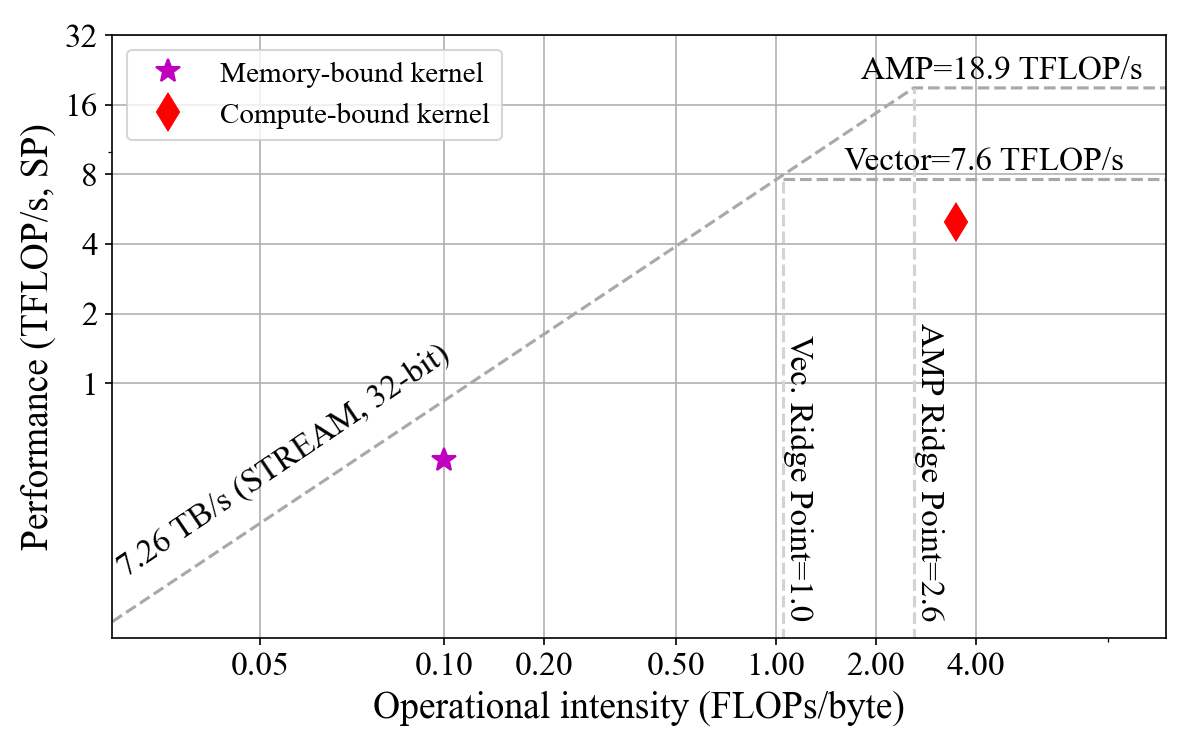
\includegraphics[width=\textwidth]{ipu-roofline-sp.png}
         \caption{32-bit precision}
         \label{fig:roofline-sp}
     \end{subfigure}
     \begin{subfigure}[b]{0.5\textwidth}
         \centering
         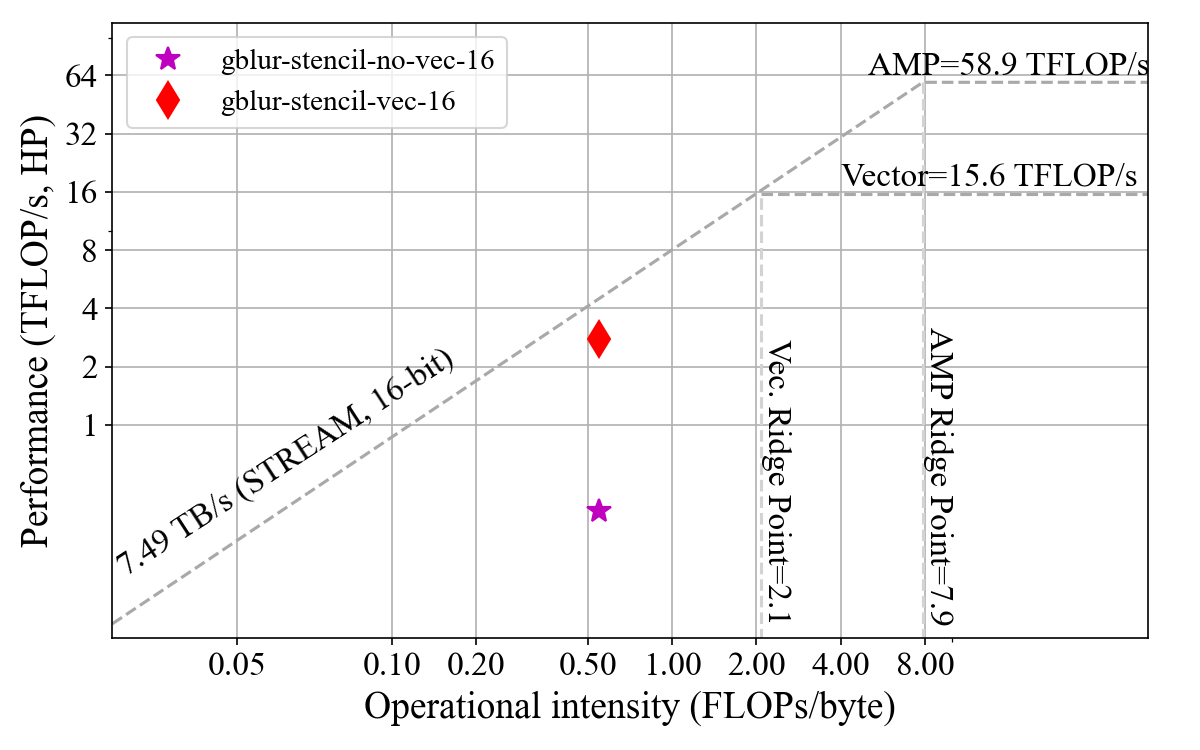
\includegraphics[width=\textwidth]{ipu-roofline-hp.png}
         \caption{16-bit precision}
         \label{fig:roofline-hp}
     \end{subfigure}
\caption{Roofline models for the IPU. For clarity, we have only plotted the performance of the largest simulation size for our Gaussian Blur and LBM stencil kernels. }
\label{fig:roofline}
\end{figure}

In this model, the y-axis represents performance attained in FLOP/s, while the x-axis represents operational intensity in FLOPs/byte -- i.e. the amount of computation performed for each byte written to or read from main memory. We plot the ceilings for the platform's memory bandwidth (determined by the STREAM benchmark) and the theoretical peak performance. We show two theoretical performance ceilings from~\cite{CitadelPaper}: the vector unit theoretical maximum, and the benchmarked matrix-multiply limit for operations that can use the AMP (Accumulating Matrix Product hardware). 32-bit and 16-bit precision have different ceilings, so we show two separate plots. 

For any given kernel, we can determine its operational intensity by counting the load/store and floating point instructions in the compiler output, and its performance by measuring the execution time over a known amount of data. 

By plotting this point on the Roofline model, we can reason about whether the kernel is memory bandwidth bound or computation bound, and can measure how close performance is to the appropriate ceiling.  The model can be used to guide the correct optimisation strategies for a given platform (e.g.~\cite{hierarchical-roofline-gpu}). 

We will use this Roofline model to discuss the performance of our example applications below, but for now we note the following:

\paragraph{Realistic expectations} Developers' hopes for IPU performance based on the theoretical limits in marketing materials should be somewhat tempered. In reality, any kernel that does not perform as least as many floating point operations as the number of bytes of memory accessed during computation is still memory bandwidth bound, and we should expect performance below 7.26 TFLOP/s for 32-bit compute. This is the limit that will apply to most HPC kernels. In fact, on other platforms, well-tuned kernels which effectively utilise caches may be able to achieve similar results to the IPU.

\paragraph{Difficulty modelling exchange and data rearrangement costs}
The STREAM triad kernels differ from most realistic vertexes for the IPU in that they do not require any data exchange between tiles (i.e. there are only local memory accesses). In practice, BSP synchronisations, inter-IPU and inter-tile exchanges, and data rearrangements specified during vertex wiring introduce costs which place a ceiling on a kernel's performance. The design choices are often in tension (e.g. better kernel performance from using aligned data comes at the cost of aligning the data before the compute phase begins).

This situation is not so different from distributed memory systems, for which Cardwell and Song extended the Roofline model with communication-awareness ~\cite{communicaton-aware-roofline}. They propose an additional visualisation showing communication limits, with a kernel characterised by a new kernel metric: \textit{communication intensity} in FLOPs/network byte, and a new platform limit in the form of a peak communication bandwidth from a benchmark. While this approach might reasonably be extended to apply to the IPU's exchange fabric, it still does not account for the data rearrangement costs before and after compute phases, which we found to far exceed communication costs. It is also impossible to accurately determine the number of bytes sent, since this is not under the control of the programmer in Poplar.

Our approach is to preserve the Roofline model's useful ability to indicate how a close a kernel is to being limited by memory bandwidth or peak compute performance by compensating proportionally for the effect of the non-compute BSP phases. Poplar's performance visualisation tooling allows us to measure the clock cycles taken in each BSP phase (in an instrumented profiling build). It is also possible to add cycle count nodes to the compute graph before and after a compute set of interest. Using this information, we can divide the execution time measured for a compute set by the fraction of time observed in the compute phase, giving us a more accurate model of what is limiting performance within a compute phase.

We also implement a ``no-op'' version of each kernel, wired into the graph in the same way as the actual kernel. By measuring the maximum rate at which cells can be updated for a given problem size with this no-op version, we can compare the costs of different data layouts, alignments and tensor transformations in isolation from the kernel.

% \paragraph{What the Roofline model does not show} The Roofline model only considers the performance of the compute phase of the BSP superstep of a kernel, but does not indicate the cost of data rearrangements and halo exchanges that may precede and succeed it. However, the cost of exchange and data rearrangement imposes a throughput ceiling that affects a kernel's achievable performance. We found that choices made for tensor transformations or memory alignment when wiring up a vertex could result in data rearrangement costs which completely dominated execution time, and were in tension with optimisations suggested by the Roofline model.

% Unfortunately, these costs vary both with the input problem size, and with implementation choices for data layout, tensor transformations and memory alignment, making them impossible to present as  platform-wide ceilings.  Still, for a given implementation and problem size, it is trivial to measure this cost by implementing a "no-op" vertex that has the same inputs and outputs as the target vertex and is wired up in the same way, but which does no work and accesses no memory. This measurement produces a throughput\footnote{A useful measure of work here is the maximum number of grid cells which can be updated per second, which in Lattice Boltzmann literature is presented in \textit{Lattice Updates Per Second} (LUP/s)} ceiling , $W$. We can convert this throughput limit into an equivalent ceiling in FLOP/s (by counting the FLOPs in the compiler output, and multiplying with $W$ and the number of cells in the grid), to determine whether $W$, rather than the memory bandwidth, forms the real performance ceiling in our implementation.

% In our example applications, we found $W$ to be well below the achievable memory bandwidth ceiling, detracting from the overall usefulness of the Roofline model for IPU development.

\section{Example applications}
\label{sec:example-applications}
\subsection{Gaussian Blur}
\label{sec:gaussian-blur}
As a first simple example of a structured grid application, we implemented the well-known 3x3 Gaussian Blur image filter. This simple filter performs a convolution of the Moore neighbourhood of a pixel with the discretised Gaussian kernel in Eq. \eqref{eq:gaussian-blur}:

\begin{equation}
\label{eq:gaussian-blur}
h = \frac{1}{16}\begin{pmatrix}
1 & 2 & 1 \\
2 & 4 & 2 \\
1 & 2 & 1
\end{pmatrix}
\end{equation}

This operation is applied to each of the  red, green, blue and alpha (RGBA) channels of the input image, resulting in a blur effect. Because the same operation is applied to the neighbourhood of each cell, the convolution can be expressed as a stencil computation.

Pixel intensities are commonly represented as 8-bit values, but for our purposes we used 32- and 16-bit numbers to better demonstrate the memory characteristics of a scientific application. We ran 200 iterations of the stencil on three test images of increasing size.

Convolutions are so commonplace in modern deep learning that the IPU contains hardware convolution units, and this example application provides an opportunity to demonstrate exploiting dedicated AI accelerator hardware vs. using hand-coded stencils.

 The graph compiler can choose from several strategies for convolutions, depending on the size and shape of inputs, and the amount of memory made available to the operation. We performed a grid search over the amount of memory allocated to this operation for our test images, and compared the best result for each image against our matrix-free stencil implementation. 
 
\begin{figure}[htbp]
\centerline{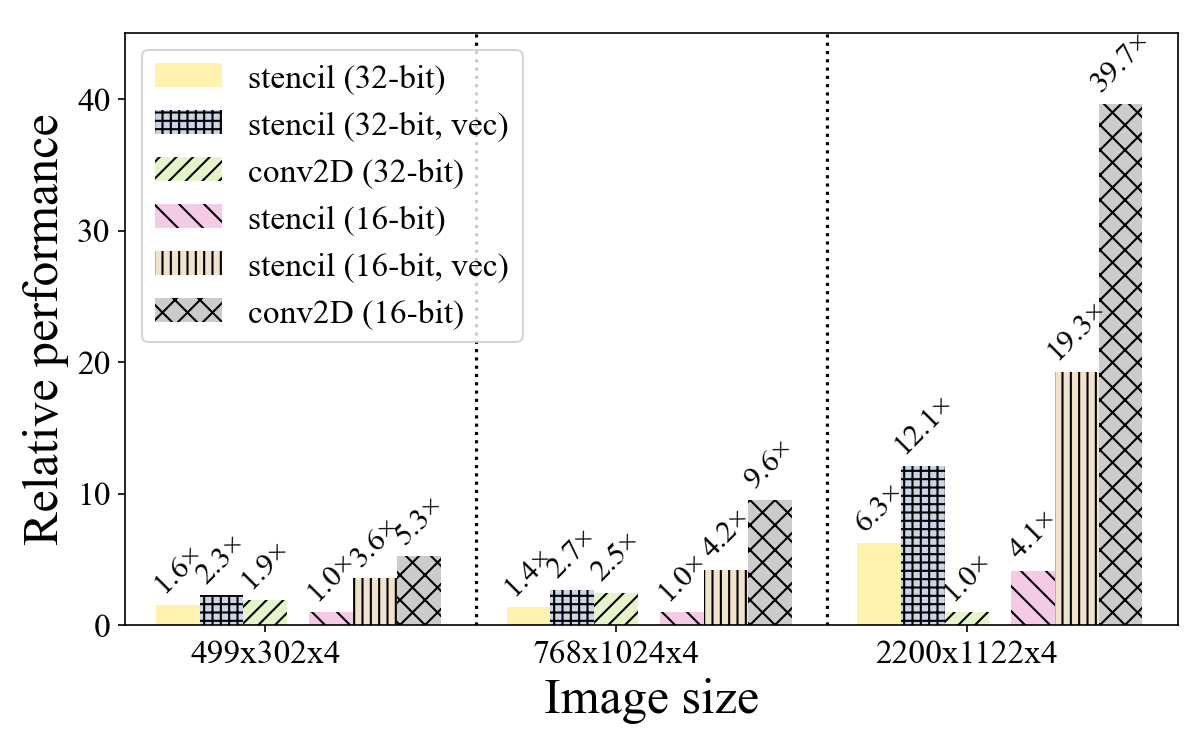
\includegraphics[width=0.5\textwidth]{gaussian-blur-precision-and-vec.png}}
\caption{Relative performance of Gaussian Blur implementations on 1 IPU (stencil and convolution) for 32-bit vs 16-bit precision, and with vectorised vs unvectorised implementations}
\label{fig:gb-datatype}
\end{figure}

  Fig.~\-\ref{fig:gb-datatype} shows that for one IPU, using the IPU's convolution hardware results in much better performance than our best stencil implementation in 16-bit precision. However, in 
  32-bit precision, our stencil implementation surprisingly outperformed the vendor-optimised convolutions.  When we scaled to 2 IPUs, more memory became available to the convolution operation, and the implementations achieved much more similar timings in 32-bit precision (stencil only 1.1x faster on the largest image). Inspecting detailed debug output from the compiler shows that the relatively large images leave insufficient memory to allow using sophisticated convolution plans on one IPU, and the compiler falls back to choosing plans that only use vector floating point instructions instead of the dedicated hardware. 
  
  Fig.~\-\ref{fig:gb-datatype} also shows vectorising the code results in significant performance improvements.
  
 We compared timings against 32-bit precision parallel implementations for CPU and GPU (details in Appendix~A).  Fig.~\- \ref{fig:gb-stencil-vs-conv} shows these results for a vectorised implementation with a single IPU, with performance normalised against the worst result.  The 1-IPU stencil implementation was consistently the best-performing for 32-bit precision. OpenCL compiler limitations meant that extensions for 16-bit precision were unavailable on the comparison platforms, precluding any comparison. 

\begin{figure}[htbp]
\centerline{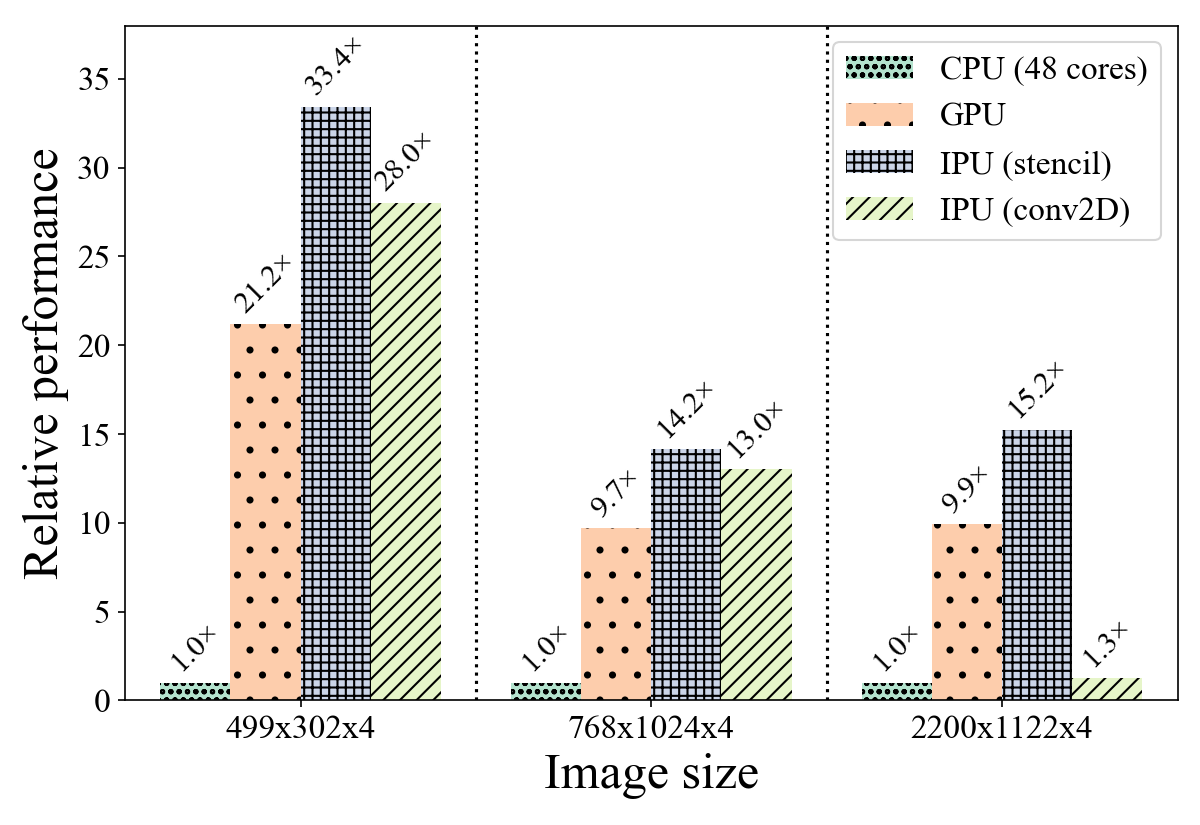
\includegraphics[width=0.5\textwidth]{gaussian-blur-relative.png}}
\caption{Relative performance of Gaussian Blur implementations on 1 IPU (stencil and convolution) vs 48 Skylake CPU cores and NVIDIA V100 GPU (32-bit, vectorised)}
\label{fig:gb-stencil-vs-conv}
\end{figure}

The Gaussian Blur kernel has a very low operational intensity (calculated from compiler output as 0.55 FLOPs/Byte, 16-bit and 0.275 FLOPs/Byte, 32-bit). At this operational intensity, the kernels are very much memory bandwidth bound according to our Roofline models in Fig.~\-\ref{fig:roofline}, with ceilings at 4.11 TFLOP/s for 16-bit precision and 2.00 TFLOP/s for 32-bit precision. Adjusted to consider the compute-phase only, our optimised stencil implementations on 1 IPU achieved 68\% (16-bit) and 88\% (32-bit) of this ceiling for the largest problem sizes, showing that it is possible to achieve an impressive fraction of peak performance. Less than 1\% of execution time was spent on halo exchange, but data rearrangement costs could account for up to 14.1\% of runtime on one IPU. When scaling up to 16 IPUs, these costs could account for more than half of the execution time, largely because of the slower inter-IPU exchange bandwidth.

\subsection{Lattice-Boltzmann Fluid Simulation}
The Lattice-Boltzmann Method (LBM) ~\cite{mcnamara-zanetti} is an increasingly popular technique for simulating fluid dynamics. In contrast to methods which solve the Navier-Stokes equations directly and methods which simulate individual particles, LBM is a mesoscopic method in which distributions of particle velocities are modelled on a discretised lattice of the domain. 

Our simple example application simulates fluid flow in a 2D lid-driven cavity, using D2Q9 discretisation, for which 9 directions of fluid flow are modelled per grid cell. 

The Lattice-Boltzmann method proceeds in two steps:
\begin{enumerate}
\item During the \textit{streaming} step, velocities from 8 cells in the immediate lattice neighbourhood are “advected” to the cell under consideration. Informally, the update rule is \textit{``my north-west neighbour’s south-east velocity becomes my new south-east velocity''}, etc. This step involves no computation, but has complex memory accesses. The regular pattern of updates from neighbours makes it is a stencil, and it  is always memory bandwidth bound.
\item During the \textit{collision} step, the directional velocity distributions are updated in a series of operations that only use local cell values. This step has simple memory accesses, but is computationally intensive.
\end{enumerate}

At each timestep, we also record the average fluid velocity, requiring a reduction over all cores.

Common optimisations for LBM implementations on multi-core CPUs and GPUs are discussed in ~\cite{lbm-optim,overview-and-derivation-of-lbm,lbm-propagation-steps,pull-algorithm,Nguyen_3.5dblocking}. The vast majority of optimisations are aimed at improving data locality (on shared memory platforms with caches), so are of little use for the IPU. Techniques to minimise memory accesses and storage requirements (e.g.~\cite{esoteric-twist}) do not easily lend themselves to Poplar's restrictions on updating the same tensor regions in one compute set. The IPU's BSP design precludes optimisations that overlap communication and computation. 
Our survey of LBM optimisation techniques yielded only vectorisation (and data layouts affecting vectorisation choices) and kernel fusion as applicable IPU optimisations.

Our fused, optimised kernel performs both the streaming and collision steps, and also calculates each worker's contribution to the total velocity, after which we must perform a series of reductions for cross-worker, cross-tile and cross-IPU calculations of the global average velocity. We use vectorised operations where possible.

We tested our implementation (32-bit only) on four problem sizes. A comparison of the execution times on 1 IPU vs our OpenCL CPU and GPU implementations is shown in Fig.~\-\ref{fig:lbm-performance}. In this case, the GPU implementation outperforms the IPU implementation for larger problem sizes, and both accelerator devices outperform the 48-core CPU implementation, owing to known limitations of the OpenCL CPU implementation  (e.g. no pinning for OpenCL work-groups to cores). The GPU version makes very good use of shared memory (at similar bandwidths to the IPU SRAM), and because our halo exchange implementation on the IPU induced data rearrangements that outweighed the benefits of the fast IPU exchange, the GPU's implementation using coalesced global memory access outperformed the IPU despite the lower HBM2 bandwidth.

\begin{figure}[htbp]
\centerline{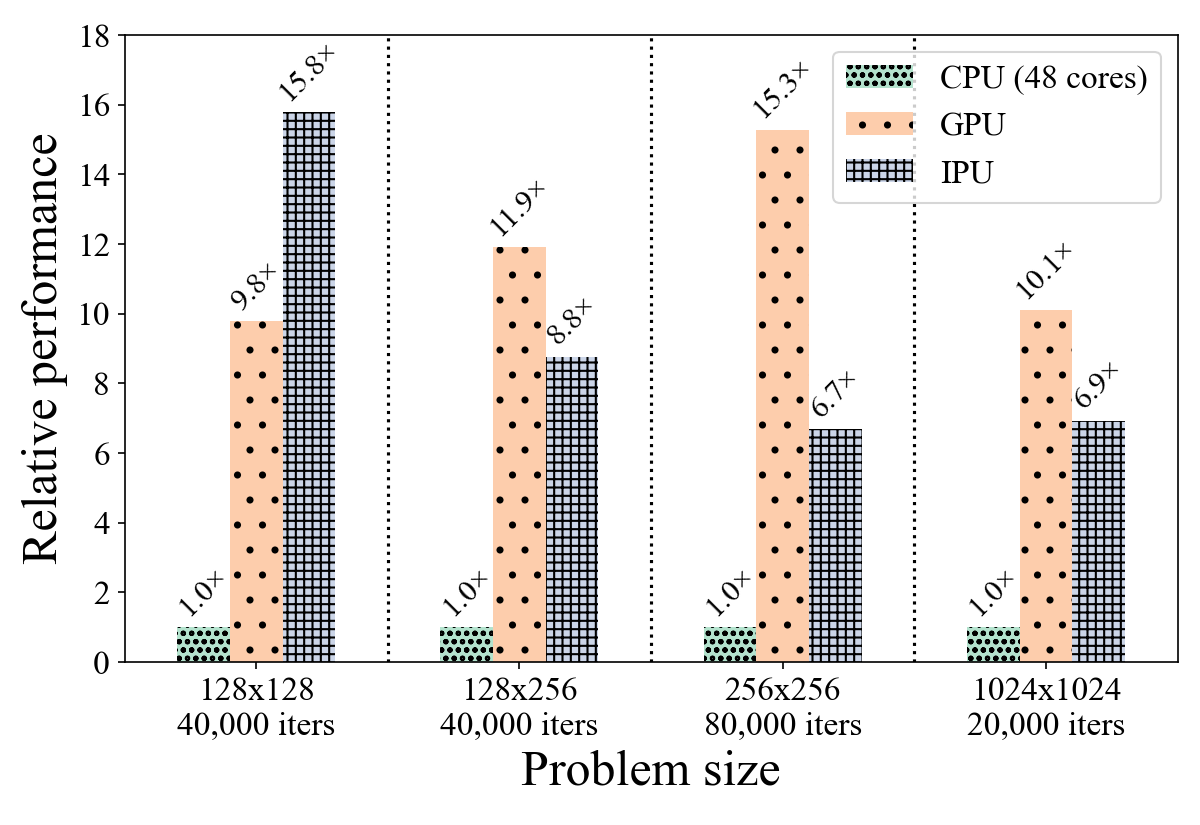
\includegraphics[width=0.5\textwidth]{lbm-relative.png}}
\caption{Relative performance of LBM D2Q9 implementations on 1 IPU vs 48 CPU cores and NVIDIA V100 GPU}
\label{fig:lbm-performance}
\end{figure}

We counted 111 FLOPs per cell update with 664 bytes of memory accesses, for an OI of 0.17 for the kernel, making it memory bandwidth bound according to our Roofline models. The high number of memory accesses on the IPU stems from its cacheless design and low number of registers compared to other platforms. 

Adjusting FLOP/s for the compute phase time, our Roofline model shows that our implementation achieved 86\% of peak performance for the largest problem size.  The smaller problem sizes only achieved around 45\% of peak performance, showing that good potential for other optimisations remains.

A BSP breakdown showed that 27\% of execution time was spent in exchange and data rearrangement activities for 1 IPU, with these costs again rising to more than 50\% of execution time on 16 IPUs.

\section{Discussion and Future Work}
We are encouraged by the promising performance seen for these two example applications on the IPU, especially in light of the years of research into optimising stencils and Lattice Boltzmann Method implementations on other platforms. Continued experience with the IPU may produce even better optimisations than our early implementations.

Our work so far has focused on structured grid applications, which find a natural expression in tensor representations, but we have also begun work with unstructured grids on the IPU for use with finite element method simulations. These require more complex representations of the sparse connections between cells and more memory accesses, but we have been able to use the graph compiler to generate efficient communication of halo regions and expect to see similar benefits as structured grid implementations from the IPU's plentiful, low-latency SRAM memory and fast exchanges.

Expressing our chosen HPC problems in Poplar was not always straightforward compared with familiar HPC technologies such as OpenMP, MPI and OpenCL. We found Poplar code to be more verbose than our OpenCL implementations ($\sim$1.6x lines of code for the Gaussian Blur stencils). 

There are important limitations in using IPU for HPC problems. Firstly, Poplar graphs are static, making it difficult to implement techniques such as dynamic grids and adaptive mesh refinement. Secondly, the graph compile time (a run-time cost) is very high compared to compilation of e.g. OpenCL kernels. For our small problems, graph compilation took longer than executing the resulting programs. Ahead-of-time compilation is also possible in Poplar. Thirdly, code developed for the IPU is not portable to other platforms. Fourthly, the IPU is limited to at most 32-bit precision, which may be insufficient for some scientific applications.

In this work, we did not consider strategies for problems that are too large to fit in the IPU's on-chip memory. We also did not measure energy use, a major reason for using AI accelerators such as the IPU in the first place. Both of these concerns are in our sights for the next phase of our research.

\section{Conclusion}
In this paper, we presented our early work on using the Graphcore IPU for traditional HPC applications. We showed that it is possible to use the IPU and its programming framework, Poplar, to express structured grid stencil computations and achieve performance comparable with modern GPUs.

Many of the techniques commonly used to optimise stencil code are inapplicable to the cacheless IPU. We also found that Roofline modelling, which characterises a kernel's performance relative to platform limits, does not show how costs associated with non-compute BSP phases might be limiting code performance. New techniques for selecting optimisations on emerging architectures may be required.

Making use of the IPU's specialised hardware, as we did for the 2D convolutions in the Gaussian Blur application, can yield large performance benefits, especially for 16-bit precision computations. Furthermore, since applications such as the ones we have implemented here are often limited by memory bandwidth, we expect many HPC applications to benefit from the large amounts of low-latency, high-bandwidth on-chip memory that chips like the IPU offer.


% \subsection{Figures and Tables}
% \paragraph{Positioning Figures and Tables} Place figures and tables at the top and 
% bottom of columns. Avoid placing them in the middle of columns. Large 
% figures and tables may span across both columns. Figure captions should be 
% below the figures; table heads should appear above the tables. Insert 
% figures and tables after they are cited in the text. Use the abbreviation 
% ``Fig.~\ref{fig}'', even at the beginning of a sentence.

% \begin{table}[htbp]
% \caption{Table Type Styles}
% \begin{center}
% \begin{tabular}{|c|c|c|c|}
% \hline
% \textbf{Table}&\multicolumn{3}{|c|}{\textbf{Table Column Head}} \\
% \cline{2-4} 
% \textbf{Head} & \textbf{\textit{Table column subhead}}& \textbf{\textit{Subhead}}& \textbf{\textit{Subhead}} \\
% \hline
% copy& More table copy$^{\mathrm{a}}$& &  \\
% \hline
% \multicolumn{4}{l}{$^{\mathrm{a}}$Sample of a Table footnote.}
% \end{tabular}
% \label{tab1}
% \end{center}
% \end{table}

% \begin{figure}[htbp]
% \centerline{
\includegraphics{fig1.png}}
% \caption{Example of a figure caption.}
% \label{fig}
% \end{figure}

% Figure Labels: Use 8 point Times New Roman for Figure labels. Use words 
% rather than symbols or abbreviations when writing Figure axis labels to 
% avoid confusing the reader. As an example, write the quantity 
% ``Magnetization'', or ``Magnetization, M'', not just ``M''. If including 
% units in the label, present them within parentheses. Do not label axes only 
% with units. In the example, write ``Magnetization (A/m)'' or ``Magnetization 
% \{A[m(1)]\}'', not just ``A/m''. Do not label axes with a ratio of 
% quantities and units. For example, write ``Temperature (K)'', not 
% ``Temperature/K''.

\section*{Acknowledgment}
The authors would like to thank Graphcore for providing access to a Dell DSS8440 Graphcore 740 16-IPU Server for this work.

\bibliography{IEEEabrv,references}

\section*{Appendix A: Platform details}
\label{app:platform-details}
\scriptsize{
\begin{itemize}
    \item Intel\textregistered~Xeon\textregistered~ Platinum 8168 (Skylake) CPUs @ 2.70GHz, 2x24 cores, 768GiB RAM
    \item IPU driver version 1.0.44, firmware version 1.3.31. Poplar SDK version v1.2.0-495c1aa368. IPU clock speed at 1.6 GHz
    \item Intel OpenCL driver v18.1.0.0920
    \item NVIDIA Volta V100 16GiB, NVIDIA CUDA Toolkit v8.0.44
    \item GCC 7.5.0 flags \texttt{-march=native -mtune=native -O3}
\end{itemize}

Comparison implementations for CPU and GPU use OpenCL v1.1. 
}


\section*{Appendix B: Example Poplar Code}
\label{app:example-vertex}
\scriptsize{
The Poplar C++ code below demonstrates a Vertex, and the use of the \texttt{half4} SIMD vector types:

\begin{lstlisting}[language=C++, frame=single, basicstyle=\scriptsize]
class GaussianBlurHalf4 : public Vertex {
public:
  // Flattened RGBA channels-last image fragments:
  // `in' includes ghost cell padding,  
  Input <Vector<half, VectorLayout::ONE_PTR, 8>> in;
  // `out' has no ghost cell padding
  Output <Vector<half, VectorLayout::ONE_PTR, 8>> out;
  // width and height are unpadded
  unsigned width;
  unsigned height;

  bool compute() {
    // Recast as half4* to make compiler 
    // generate 64-bit loads and stores
    const auto h4in = reinterpret_cast<half4 *>(&in[0]);
    auto h4out = reinterpret_cast<half4 *>(&out[0]);

    // Vectorised: each variable represents 4 halfs
    // So each operation works on 4 values
    // We do one RGBA pixel (all channels) per iteration
    for (auto y = 0; y < height; y++) {
        for (auto x = 0; x < width; x++) {
            #define H4_IDX(ROW, COL) \
                (width+2)*((y+1)+ROW)+((x+1)+COL)

            const auto nw = h4in[H4_IDX(-1, -1)];
            const auto w  = h4in[H4_IDX( 0, -1)];
            const auto sw = h4in[H4_IDX(+1, -1)];
            const auto n  = h4in[H4_IDX(-1,  0)];
            const auto m  = h4in[H4_IDX( 0,  0)];
            const auto s  = h4in[H4_IDX(+1,  0)];
            const auto ne = h4in[H4_IDX(+1, +1)];
            const auto e  = h4in[H4_IDX( 0, +1)];
            const auto se = h4in[H4_IDX(-1, +1)];
            h4out[width * y + x] =  
                1.f/16 * (nw+ne+sw+se) +
                4.f/16 * m + 
                2.f/16 * (e+w+s+n);
        }
    }
    return true;
  }
};
\end{lstlisting}

The following snippet demonstrates how a Vertex is added to the graph and mapped to a tile:


\begin{lstlisting}[language=C++, frame=single, basicstyle=\scriptsize]
auto graph = poplar::Graph(ipuDevice);
...
// Omitted for brevity: 
// Tensors are declared and partitioned over tiles
// Some tensor slices are defined: 'someTensorSliceWithHalos' 
// (mostly on tile 123, with borders on neighbouring tiles);
// 'someTensorSliceNoHalos' (wholly contained on tile 123) 
...
// Load the file containing the vertex code
graph.addCodelets("GaussianBlurCodelets.cpp",
    CodeletFileType::Auto, 
    "-O3");
// Create a compute set (BSP phase)
auto cs = graph.addComputeSet("Example Compute Set");
// Add vertex to the graph, wiring up to tensor slices
auto v = graph.addVertex(
  cs,
  "GaussianBlurHalf4",
  {
    {"in",  someTensorSliceWithHalos.flatten()},
    {"out", someTensorSliceNoHalos.flatten()},
  });
graph.setInitialValue(v["width"], width);
graph.setInitialValue(v["height"], height);
graph.setTileMapping(v, 123); // Place vertex on tile 123
...
\end{lstlisting}

}


\end{document}
